\chapter{Early-stage research work: Sinc Kolmogorov-Arnold neural network and its applications in physics-informed neural network}

\section{Introduction}\label{section:introduction}
The multilayer perceptron (MLP) represents a foundational architecture in neural networks, characterized by fully connected layers incorporating nonlinear activation functions through function superposition. The seminal Kolmogorov-Arnold representation theorem \citep{kolmogorov1961representation,arnol1959representation} demonstrates that any continuous function can be represented through the superposition of functions with at most two variables, thereby establishing a theoretical foundation for research into learnable activation functions.

The development of Kolmogorov's Spline Network (KSN) \citep{igelnik2003kolmogorov} introduced a two-layer framework utilizing splines as learnable activation functions. Recent advances in Kolmogorov-Arnold Networks (KANs) \citep{liu2024kan} have reinvigorated interest in these approaches by proposing a multilayer variant of KSN. This framework demonstrates that any successful basis for univariate function representation can generate a new KAN variant. Researchers have extensively investigated numerous basis functions, including wavelets \citep{bozorgasl2024wav,seydi2024unveiling}, Fourier series \citep{xu2024fourierkan}, finite basis functions \citep{howard2024finite}, Jacobi basis functions \citep{aghaei2024fkan}, polynomial basis functions \citep{seydi2024exploring}, rational functions \citep{aghaei2024rkan}, and Chebyshev polynomials \citep{ss2024chebyshev,shukla2024comprehensive}.

This research proposes the implementation of Sinc interpolation, defined in Equation~\ref{eq:sinc}, which has demonstrated remarkable efficacy in function interpolation, particularly for one-dimensional problems \citep{stenger2016handbook}. To our knowledge, the application of Sinc interpolation within the KAN framework remains unexplored. We posit that Sinc interpolation should supersede the cubic spline interpolation currently employed in KANs, as splines excel primarily in approximating analytic functions without singularities, a domain where MLPs already demonstrate competence. In contrast, Sinc methods exhibit superior performance in addressing problems involving singularities, boundary-layer phenomena, and infinite or semi-infinite ranges \citep{stenger2012numerical}. The integration of Sinc functions has the potential to enhance both the accuracy and generalization capabilities of KANs, particularly in addressing these challenging mathematical problems within machine learning frameworks. Our numerical experiments provide empirical validation of this hypothesis.

Physics-informed neural networks (PINNs) \citep{lagaris1998artificial,raissi2019physics} represent an innovative approach to solving partial differential equations by integrating physical laws within neural network architectures. Recent research has explored the implementation of KANs within PINNs, leading to the development of Physics-Informed Kolmogorov-Arnold Networks (PIKANs) \citep{rigas2024adaptive,wang2024kolmogorov}. Due to the architectural similarities between KANs and MLPs, PIKANs inherit several advantageous characteristics of PINNs, including their ability to mitigate the curse of dimensionality \citep{wojtowytsch2020can,han2018solving}, handle imperfect data \citep{karniadakis2021physics}, and perform interpolation \citep{sliwinski2023mean}.

The applications of PINNs span diverse domains, including fluid dynamics \citep{raissi2020hidden,jin2021nsfnets,kashefi2022physics}, quantum mechanical systems \citep{jin2022physics}, surface physics \citep{fang2019physics}, electric power systems \citep{nellikkath2022physics}, and biological systems \citep{yazdani2020systems}. However, these methods face several challenges, including spectral bias \citep{xu2019frequency,wang2022and}, error estimation complexities \citep{fanaskov2024astral}, and scalability limitations \citep{yao2023multiadam}.

This research introduces a novel neural network architecture, the Sinc Kolmogorov-Arnold Networks (SincKANs). This innovative approach leverages Sinc interpolation's exceptional capability in approximating functions with singularities to enhance the learnable activation functions traditionally employed in KANs. The improved handling of singularities enables SincKAN to effectively mitigate the spectral bias observed in PIKANs, thereby enhancing their robustness in solving partial differential equations that conventional PINNs struggle to address. We present comprehensive experimental validation of SincKAN's interpolation capabilities and evaluate their effectiveness as alternatives to traditional MLPs and KANs within the PINN framework.

The primary contributions of this research can be summarized as follows:
\begin{enumerate}
    \item Development of Sinc Kolmogorov-Arnold Networks, a novel architecture specifically designed for robust handling of singularities
    \item Introduction of multiple enhancement strategies derived from classical Sinc methods to improve SincKAN's robustness and performance
    \item Comprehensive experimental validation demonstrating SincKAN's effectiveness in function approximation and PINN applications
\end{enumerate}

The remainder of this chapter is organized as follows: Section~\ref{Section: Methods} presents a comprehensive overview of PINNs, examines Sinc numerical methods, and provides a detailed exposition of SincKAN. Section~\ref{Section: experiments} presents comparative analyses of SincKAN against several neural network architectures, including MLPs, modified MLPs \citep{wang2021understanding}, KANs, and ChebyKANs, across diverse benchmarks encompassing smooth functions, discontinuous functions, and boundary layer problems. Section~\ref{Section: conclusion} synthesizes our findings and discusses remaining challenges and future research directions.

\section{Methodological Framework}\label{Section: Methods}
\subsection{Physics-Informed Neural Networks}
We begin with a systematic examination of physics-informed neural networks (PINNs) \citep{raissi2019physics} in the context of partial differential equation (PDE) solution inference. The general form of time-dependent PDEs for $\boldsymbol{u}$ can be expressed as:
\begin{equation}
\begin{aligned}
    & \partial_{t}\boldsymbol{u}+\mathcal{N}[\boldsymbol{u}]=0, \quad t \in[0, T],\ \boldsymbol{x} \in \Omega, \\
    & \boldsymbol{u}(0, \boldsymbol{x})=\boldsymbol{g}(\boldsymbol{x}), \quad \boldsymbol{x} \in \Omega, \\
    & \mathcal{B}[\boldsymbol{u}]=0, \quad t \in[0, T],\ \boldsymbol{x} \in \partial \Omega,
\end{aligned}\label{PDE}
\end{equation}
where $\mathcal{N}$ represents the differential operator, $\Omega$ denotes the domain of grid points, and $\mathcal{B}$ signifies the boundary operator. For time-independent PDEs, we have $\partial_{t}\boldsymbol{u}\equiv 0$. 

The fundamental objective of PINNs is to approximate the unknown solution $\boldsymbol{u}$ to the PDE system defined in Equation~\ref{PDE} through the optimization of a neural network $\boldsymbol{u}^{\theta}$, where $\theta$ represents the trainable parameters. The loss function is constructed as:
\begin{equation}\label{PINN}
\mathcal{L}(\theta)=\mathcal{L}_{ic}(\theta)+\mathcal{L}_{bc}(\theta)+\mathcal{L}_r(\theta),
\end{equation}
where the individual components are defined as:
\begin{equation}
\begin{aligned}
& \mathcal{L}_r(\theta)=\frac{1}{N_r} \sum_{i=1}^{N_r}\left|\partial_{t}\boldsymbol{u}^\theta\left(t_r^i, \boldsymbol{x}_r^i\right)+\mathcal{N}\left[\boldsymbol{u}^\theta\right]\left(t_r^i, \boldsymbol{x}_r^i\right)\right|^2,\\
& \mathcal{L}_{ic}(\theta)=\frac{1}{N_{ic}} \sum_{i=1}^{N_{ic}}\left|\boldsymbol{u}^\theta\left(0, \boldsymbol{x}_{ic}^i\right)-\boldsymbol{g}\left(\boldsymbol{x}_{ic}^i\right)\right|^2, \\
& \mathcal{L}_{bc}(\theta)=\frac{1}{N_{bc}} \sum_{i=1}^{N_{bc}}\left|\mathcal{B}\left[\boldsymbol{u}^\theta\right]\left(t_{bc}^i, \boldsymbol{x}_{bc}^i\right)\right|^2.
\end{aligned}
\end{equation}

These terms correspond to the three equations in System~\ref{PDE}, where $\boldsymbol{x}_{ic}^i$, $\boldsymbol{x}_{bc}^i$, and $\boldsymbol{x}_{r}^i$ represent sampled points from the initial constraint, boundary constraint, and residual constraint, respectively. The parameters $N_{ic}$, $N_{bc}$, and $N_r$ denote the corresponding total number of sampled points for each constraint. It should be noted that in the original formulation \citep{raissi2019physics}, $u^\theta\left(x\right)=\mathbf{MLP}\left(x\right)$.


\subsection{Sinc Numerical Methods}\label{section: sinc_numerical_methods}
The Sinc function, fundamentally defined as\footnote{In engineering applications, the Sinc function is conventionally defined as $\mathrm{Sinc}(x)=\frac{\sin(\pi x)}{\pi x}$}
\begin{equation}\label{eq:sinc}
    \mathrm{Sinc}(x)=\frac{\sin(x)}{x},
\end{equation}
serves as the foundation for our numerical approach. The Sinc series $S(j, h)(x)$ employed in Sinc numerical methods is expressed as:
\begin{equation}\label{candidate function}
S(j, h)(x)=\frac{\sin [(\pi / h)(x-j h)]}{(\pi / h)(x-j h)},    
\end{equation}
which enables the Sinc approximation for a function $f$ defined on the real line $\mathbb{R}$:
\begin{equation}\label{eq: sinc_approx}
f(x) \approx \sum_{j=-N}^N f(j h) S(j, h)(x), \quad x \in \mathbb{R}.
\end{equation}
Here, $h$ represents the step size with the optimal value $\sqrt{\pi d/\beta N}$ as established in Theorem~\ref{Theorem: Stenger}, and $2N+1$ denotes the degree of the Sinc series.

The Sinc function's remarkable properties, including its equivalence to the semidiscrete Fourier transform \citep{trefethen2000spectral} and its approximation as a nascent delta function, have established Sinc numerical methods as a powerful technique for addressing diverse linear and nonlinear problems in scientific and engineering applications. These applications span various domains, including heat transfer \citep{lippke1991analytical}, fluid mechanics \citep{abdella2015solving}, and solid mechanics \citep{abdella2009application}. 


However, the actual implementation of Sinc numerical methods has a key difficulty: Sinc series constitute orthogonal bases defined on $(-\infty,\infty)$, which presents complications for numerical applications. Effective implementation requires both an appropriate coordinate transformation based on the computing domain $(a,b)$ and an optimal step size calibrated to the target function $f$. Manual adjustment of network parameters for each specific problem proves impractical and inefficient. We first present the classical techniques employed in Sinc numerical methods before discussing their adaptation to machine learning applications in Section~\ref{Section: sinckan}. 

The convergence properties of Sinc approximation are formalized in the following theorem:

\begin{theorem}\label{Theorem: Stenger} \citep{sugihara2004recent}
Let $\alpha, \beta, d >0$. Assume that:

(1) $f$ belongs to $H^1(\mathcal{D}_d)$, where $H^1$ denotes the Hardy space and $\mathcal{D}_d=\{z\in \mathbb{C} \mid |\Im z|<d\}$;

(2) $f$ exhibits exponential decay on the real line, satisfying $|f(x)| \leq \alpha \exp (-\beta|x|)$ for all $x \in \mathbb{R}$.

Then there exists a constant $C$ such that:
\begin{equation}
\sup _{-\infty<x<\infty}|f(x)-\sum_{j=-N}^N f(j h) S(j, h)(x)| \leq C N^{1/2} \exp [-(\pi d \beta N)^{1/2}],   
\end{equation}
where the optimal step size $h$ is given by:
\begin{equation}\label{optimal_h}
h=\left(\frac{\pi d}{\beta N}\right)^{1/2}.    
\end{equation}
\end{theorem}

Theorem~\ref{Theorem: Stenger} demonstrates that the exponential convergence of Sinc approximation on the real line depends critically on the parameters $d$ and $\beta$, which are determined by the target function $f$. In traditional Sinc numerical methods, researchers either specify parameters for particular functions \citep{sugihara2004recent,mohsen2017accurate} or employ bisection methods \citep{richardson2011sinc}. Both approaches necessitate knowledge of the target function $f$, which is typically unavailable in machine learning applications.

Practical numerical applications generally require approximation on a finite interval $(a,b)$ rather than the entire real line $\mathbb{R}$. Implementation of Sinc methods for general functions necessitates a transformation from the interval $(a, b)$ to $\mathbb{R}$ through an appropriately selected coordinate transformation $\psi(\xi)$, where $\psi: (-\infty,+\infty) \rightarrow (a,b)$. This transforms Equation~\ref{eq: sinc_approx} into:
\begin{equation}\label{eq: sinc_approx_trans}
f(\psi(\xi)) \approx \sum_{j=-N}^N f(\psi(j h)) S(j, h)(\xi), \quad -\infty<\xi<\infty,
\end{equation}
where $h$ maintains its optimal value $\sqrt{\pi d^\prime/\beta^\prime N}$ as established in Theorem~\ref{Theorem: transformation}.

The preservation of convergence properties under coordinate transformation is established by the following theorem:

\begin{theorem} \label{Theorem: transformation} \citep{sugihara2004recent}
For a variable transformation $x=\psi(\xi)$, assume that the transformed function $f(\psi(\xi))$ satisfies conditions (1) and (2) of Theorem~\ref{Theorem: Stenger} with parameters $\alpha^\prime$, $\beta^\prime$, and $d^\prime$. Then there exists a constant $C$ such that:
\begin{equation}
\sup _{a \leq x \leq b}|f(x)-\sum_{j=-N}^N f(\psi(j h)) S(j, h)(\psi^{-1}(x))| \leq C N^{1/2} \exp [-(\pi d^\prime \beta^\prime N)^{1/2}],
\end{equation}
where the optimal step size is given by:
\begin{equation}
h=\sqrt{\frac{\pi d^\prime}{\beta^\prime N}}.
\end{equation}
\end{theorem}

This theorem presents a significant finding: through appropriate choice of transformation, even functions exhibiting end-point singularities can be successfully approximated using Equation~\ref{eq: sinc_approx_trans}. To demonstrate the practical advantages of Sinc methods, we present empirical results in Figure~\ref{fig:matlab}, generated using Chebfun \citep{driscoll2014chebfun} for Chebyshev and cubic spline interpolation, and Sincfun \citep{richardson2011sinc} for Sinc interpolation.

\begin{figure}[ht]
   \centering
    \subfigure[\label{sqrt_matlab}Function $f(x)=\sqrt{x}$]{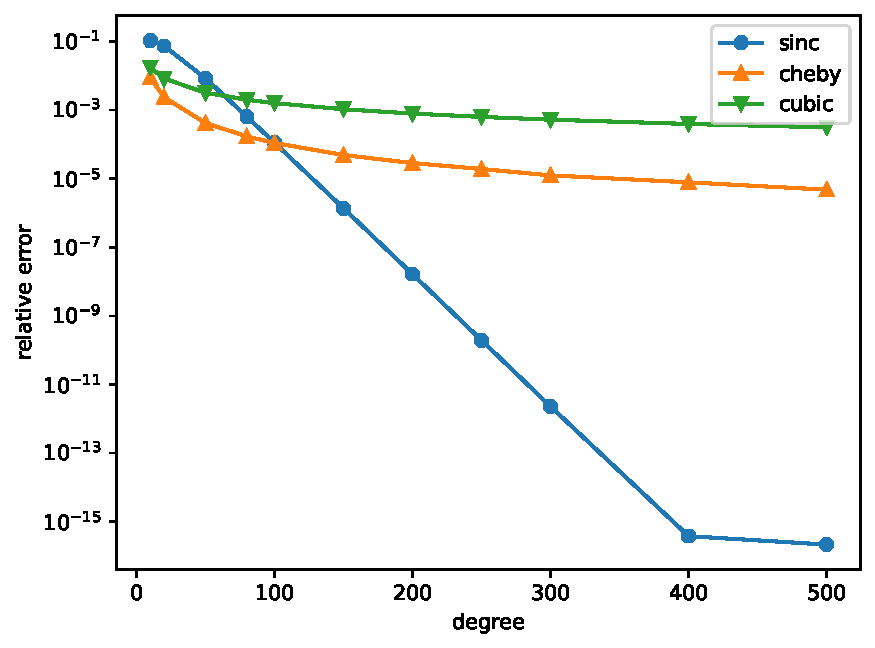
\includegraphics[width=0.3\linewidth]{ThesisFigs/sqrt_matlab.pdf}}
    \subfigure[\label{bl_matlab}Function $f(x)=e^{-10^5x}$]{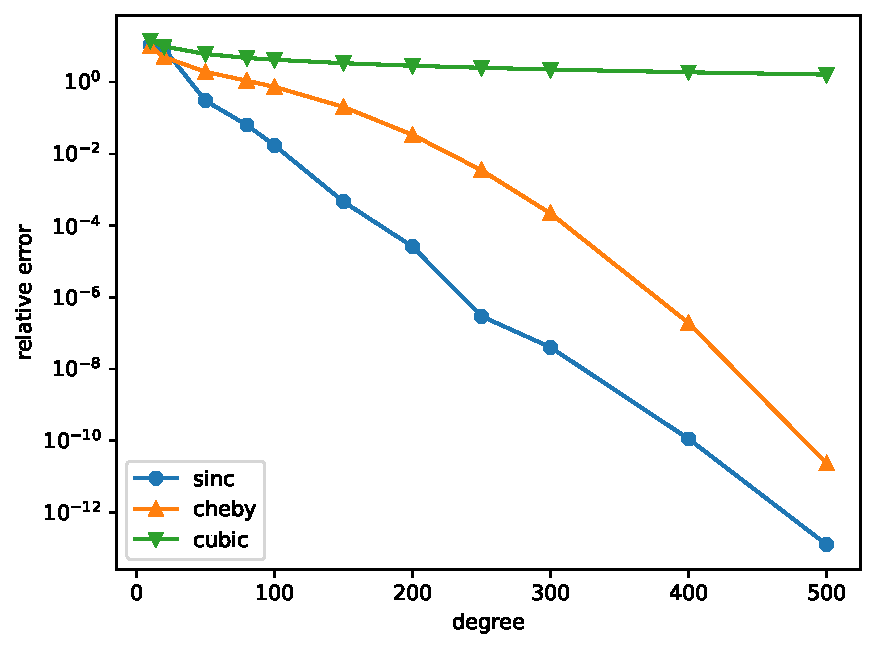
\includegraphics[width=0.3\linewidth]{ThesisFigs/bl10000_matlab.pdf}}
    \subfigure[\label{bl10000_solution}Comparative analysis of \ref{bl_matlab}]{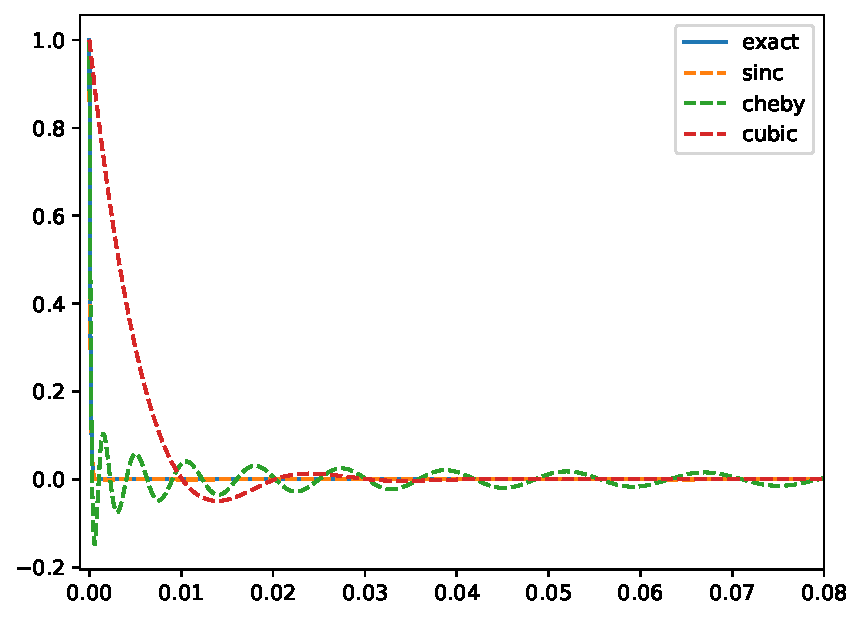
\includegraphics[width=0.3\linewidth]{ThesisFigs/bl10000_solution.pdf}}
   \caption{Comparative analysis of interpolation methods: (a) demonstrates Sinc's superior performance in handling end-point singularities, contrasting with the slower convergence of Chebyshev and spline methods; (b) illustrates exponential convergence of Sinc methods for boundary layer functions with high derivatives, while Chebyshev methods exhibit initial slow convergence; (c) presents detailed solution comparisons over $[0,0.08]$, highlighting Sinc interpolation's superior accuracy against Chebyshev's oscillatory behavior and spline's localized inaccuracies.}
    \label{fig:matlab}
\end{figure}

\subsection{Sinc Kolmogorov-Arnold Network Architecture}\label{Section: sinckan}
Consider a matrix of univariate functions $\mathbf{\Phi}=\{\phi_{p,q}\}$ where $p= 1, 2, \dots n_{in}$ and $q= 1, 2, \dots n_{out}$. The L-layer Kolmogorov-Arnold Network can be formally defined as\footnote{A comprehensive explanation of KAN architecture is provided in Appendix~\ref{Appendix: networks_kan}}:
\begin{equation}
    \mathrm{KAN} (\vx) = (\mathbf{\Phi}_{L-1} \circ \mathbf{\Phi}_{L-2} \circ \cdots \circ \mathbf{\Phi}_1 \circ \mathbf{\Phi}_0) \vx, \quad \vx\in \mathbb{R}^d.
\end{equation}

In the canonical KAN formulation \citep{liu2024kan}, each univariate function $\phi$ is approximated through a summation incorporating cubic spline interpolation:
\begin{equation}
    \phi_{\mathrm{spline}}(x)=w_b \mathrm{silu}(x)+w_s \left(\sum_i c_i B_i(x)\right),
\end{equation}
where $c_i$, $w_b$, and $w_s$ represent trainable parameters, and $B_i$ denotes the spline basis function. A natural extension to incorporate Sinc interpolation would be:
\begin{equation}\label{eq: old_sinckan}
    \phi_{\mathrm{single}}(x) = \sum_{i=-N}^N c_{i} S(i, h)(x),
\end{equation}
where $c_i$ represents trainable parameters. When $h$ is set to the optimal value given by Equation~\ref{optimal_h}, the optimal approximation of $f(x)$ in Equation~\ref{eq: sinc_approx} is achieved when $c_i^*=f(ih)$ for all $i=-N,\dots,N$. But several technical problems need to be taken into account when putting this algorithm into practice:

\paragraph{Optimal Step Size Selection}
The determination of optimal step size presents a significant challenge in machine learning frameworks, as discussed in Section~\ref{section: sinc_numerical_methods}. To address this limitation, we propose an extension to the Sinc approximation that incorporates multiple step sizes $h_j$:
\begin{equation}
    \phi_{\mathrm{multi}}(x) = \sum_{j=1}^{M}\sum_{i=-N}^N c_{i,j} S(i, h_j)(x),
\end{equation}
where $c_{i,j}$ represents the trainable parameters. Previous research \citep{stenger2012numerical} has established that step sizes larger than the optimal value predicted by Equation~\ref{optimal_h} yield improved accuracy at points distant from the origin while sacrificing precision near the origin. Conversely, smaller step sizes enhance accuracy near the origin while reducing precision at distant points. Therefore, the combination of different step sizes with adaptive weights can potentially achieve a superior approximation compared to using a single optimal step size, while eliminating the need for explicit optimal step size calculation. This expansion of the approximation through multiple step sizes $h_j$ not only circumvents the need for problem-specific step size determination but also enhances overall accuracy.

\paragraph{Coordinate Transformation Implementation}
Another significant challenge lies in the selection of appropriate coordinate transformations, which traditionally requires problem-specific optimization \citep{stenger2000summary}. Let $\mathcal{X}=\{x_i\}_{i=1}^{N}$ denote an ordered set of input points where $x_1 \leq x_2 \leq \cdots \leq x_N$. We can define the open interval $(a,b)$ as $a=x_1-\epsilon, b=x_N+\epsilon$, where $\epsilon$ represents a chosen margin, and $\xi_1=\psi^{-1}(x_1),\xi_N=\psi^{-1}(x_N)$. This transformation maps the input interval from $[x_1,x_N]$ to $[\xi_1,\xi_N]$. However, applying such transformations at each sub-layer leads to increasing and inconsistent input scales, potentially impeding network convergence \citep{ioffe2015batch}. 

To address this scaling issue, we propose that input normalization at each layer is essential. Previous research \citep{bozorgasl2024wav} has demonstrated the effectiveness of batch normalization \citep{ioffe2015batch} in enhancing KAN performance. In our SincKAN architecture, we introduce a normalizing transformation $\phi(x)=\frac{x-\mu}{\sigma}$, where $\sigma$ represents the scaling factor and $\mu$ denotes the shifting factor. The composition of $\phi$ and $\psi$ satisfies the conditions for $\psi$ specified in Theorem~\ref{Theorem: transformation}, and the transformed function $f(\psi \circ \phi^{-1}(\xi))$ maintains compliance with assumptions (1) and (2) in Theorem~\ref{Theorem: Stenger} under modified parameters $\alpha^{\star}$, $\beta^\star$, and $d^\star$ (proof provided in Appendix~\ref{Appendix: theorem 3}). Consequently, the optimal step size becomes $\sqrt{\pi d^\star/\beta^\star N}$.

We define the normalized coordinate transformation $\gamma^{-1}(x) := \phi \circ \psi^{-1}(x)$ such that $\gamma^{-1}: (a,b) \rightarrow (-\infty,\infty)$ and $[x_1,x_N] \rightarrow [\frac{\xi_1-\mu}{\sigma},\frac{\xi_N-\mu}{\sigma}]$, where $\sigma$ and $\mu$ satisfy $[\frac{\xi_1-\mu}{\sigma},\frac{\xi_N-\mu}{\sigma}] \subset [-1,1]$. This normalized transformation $\gamma$ supersedes the traditional coordinate transformation $\psi$ in our SincKAN implementation. The adaptation of optimal step size $h$ to different values of $\sigma$ and $\mu$ is facilitated by the summation of different $h_j$, allowing us to maintain consistency with the fixed scale $[-1,1]$ by defining the set $\{h_j\}$ relative to this domain, independent of specific $\sigma$ and $\mu$ values.

\paragraph{Exponential Decay Condition}
Theorem~\ref{Theorem: transformation} imposes an exponential decay condition requiring $f(-\infty)=f(+\infty)=0$. To extend Sinc methods to general functions, \citep{richardson2011sinc} proposes interpolating the difference $g-f$ rather than $f$ directly, where $g$ represents a linear function matching $f$ at the endpoints. In our SincKAN architecture, we implement this concept through a learnable linear function serving as a skip-connection for difference approximation.

Integrating these three methodological innovations, we define our learnable activation function in SincKAN as:
\begin{equation}\label{eq: Sinc activation function}
    \phi_{\mathrm{sinc}}(x) = c_1x+c_2+ \sum_{j=1}^{M}\sum_{i=-N}^N c_{i,j} S(i, h_j)(\gamma^{-1}(x)),
\end{equation}
where $c_1$, $c_2$, and $c_{i,j}$ represent learnable parameters, $S$ denotes the Sinc function, and $\gamma$ represents the normalized transformation.

\section{Experimental Validation}\label{Section: experiments}
This section presents a comprehensive evaluation of SincKAN's performance through a series of carefully designed experiments encompassing function approximation and PDE solution tasks. We compare SincKAN against several representative neural network architectures: the classical Multilayer Perceptron (MLP) commonly employed in PINNs; Modified MLP, which enhances hidden layer capability through high-dimensional feature space projection \citep{wang2021understanding}; the original KAN architecture; and ChebyKAN, which leverages Chebyshev polynomials' approximation capabilities and has been extensively validated in previous research \citep{shukla2024comprehensive}.

In our implementation, we employ the hyperbolic tangent function for the normalized transformation $\gamma(x)=\tanh(x)$ and incorporate a linear skip connection with parameters $w_1 \in \mathbb{R}^{n_{in}\times n_{out}}$ and $w_2 \in \mathbb{R}^{n_{out}}$. It is noteworthy that we observed the instability in ChebyKAN implementation previously reported by \citep{shukla2024comprehensive}; consequently, our experiments utilize the modified ChebyKAN variant proposed in their work, which incorporates a hyperbolic tangent activation function between layers. Detailed architectural specifications and hyperparameter configurations are provided in Appendices~\ref{Appendix: networks} and \ref{Appendix: expeirment details}, respectively.

\subsection{Function Approximation Analysis}
Function approximation represents a fundamental objective of KANs, with significant applications in feature identification, modular structure discovery, and symbolic formula extraction \citep{liu2024kan2}. Moreover, the neural network training process can be conceptualized as approximating mappings between complex functional spaces, making approximation accuracy a direct indicator of network capability. Therefore, we begin our experimental validation with approximation tasks to demonstrate SincKAN's competence and establish its viability as a competitive architecture. To maintain consistency with previous KAN research, we employ the Root Mean Square Error (RMSE) as our primary evaluation metric.

While Sinc numerical methods have established theoretical and empirical superiority in handling singularities, we posit that SincKAN's applicability extends beyond traditional numerical methods to general machine learning scenarios. To demonstrate this robustness, we conducted extensive experiments across both smooth functions (where cubic spline interpolation traditionally excels) and functions with singularities (where Sinc interpolation demonstrates advantages). Table~\ref{table: function approxmation} presents a subset of these results, with complete results available in Table~\ref{table: function approxmation rest}. Detailed function specifications are provided in Appendix~\ref{Appendix: details of approximate functions}.

\begin{table}[ht]
\caption{RMSE of functions for approximation}
\label{table: function approxmation}
\begin{center}
\begin{adjustbox}{width=\columnwidth, center}
\begin{tabular}{llllll}
\multicolumn{1}{c}{\bf Function name}  & \multicolumn{1}{c}{\bf MLP} & \multicolumn{1}{c}{\bf modified MLP} &\multicolumn{1}{c}{\bf KAN} & \multicolumn{1}{c}{\bf ChebyKAN} & \multicolumn{1}{c}{\bf SincKAN (ours)} 
\\ \hline 
\textit{sin-low} & $1.51 e\mbox{-}2 \pm 2.01 e\mbox{-}2$ & $7.29e\mbox{-}4 \pm 2.98 e\mbox{-}4$ & $1.27e\mbox{-}3 \pm 3.13e\mbox{-}4$ &
$1.76e\mbox{-}3 \pm 3.19e\mbox{-}4$ &
\textcolor{red}{$3.55 e\mbox{-}4 \pm 3.08 e\mbox{-}4$} \\ 
\textit{sin-high} & $7.07e\mbox{-}1 \pm 6.44e\mbox{-}8$ & $7.07 e\mbox{-}1 \pm 1.15 e\mbox{-}5$ & $7.06e\mbox{-}1 \pm 1.36e\mbox{-}3$ &
$5.70e\mbox{-}2 \pm 5.99 e\mbox{-}3$ &
\textcolor{red}{$3.94e\mbox{-}2 \pm 5.36e\mbox{-}3$} \\ 
\textit{multi-sqrt} & $2.06e\mbox{-}3 \pm 1.16e\mbox{-}3$ & $4.59e\mbox{-}4 \pm 4.86e\mbox{-}4$ & $3.61e\mbox{-}4 \pm 8.67 e\mbox{-}5$ &
$2.34e\mbox{-}3 \pm 1.17e\mbox{-}3$ &
\textcolor{red}{$2.14e\mbox{-}4 \pm 2.49 e\mbox{-}4$} \\ 
\textit{piece\mbox{-}wise} & $2.01e\mbox{-}2 \pm 5.16e\mbox{-}3$ & $3.76e\mbox{-}2 \pm 1.83e\mbox{-}2$ & $5.84e\mbox{-}2 \pm 1.03e\mbox{-}2$ &
$7.28e\mbox{-}3 \pm 9.59 e\mbox{-}4$ &
\textcolor{red}{$2.14e\mbox{-}3 \pm 7.76e\mbox{-}4$} \\ 
\textit{spectral-bias} & $4.18e\mbox{-}3 \pm 1.18 e\mbox{-}3$ & $1.59e\mbox{-}3 \pm 2.39e\mbox{-}4$ & $4.73e\mbox{-}2 \pm 9.94 e\mbox{-}3$ &
$5.60e\mbox{-}3 \pm 2.56 e\mbox{-}4$ &
\textcolor{red}{$1.48e\mbox{-}3 \pm 1.82 e\mbox{-}4$} \\
\textcolor{blue}{\textit{multimodal2-2d}} & $7.55e\mbox{-}3 \pm 2.59 e\mbox{-}3$ & $2.43e\mbox{-}3 \pm 1.15e\mbox{-}3$ & $7.97e\mbox{-}3 \pm 4.82 e\mbox{-}3$ &
$6.12e\mbox{-}2 \pm 2.02e\mbox{-}2$ &
\textcolor{red}{$2.11e\mbox{-}3 \pm 3.57e\mbox{-}4$} \\
\textcolor{blue}{\textit{fractal-2d}} & $2.89e\mbox{-}2 \pm 2.40 e\mbox{-}2$ & $2.60e\mbox{-}2 \pm 7.26e\mbox{-}3$ & $2.54e\mbox{-}1 \pm 1.88 e\mbox{-}2$ &
$6.14e\mbox{-}2 \pm 5.07e\mbox{-}3$ &
\textcolor{red}{$7.53e\mbox{-}3 \pm 6.09e\mbox{-}4$} \\
\textcolor{blue}{\textit{lpmv}} & $1.27e\mbox{-}3 \pm 6.13 e\mbox{-}5$ & $3.79e\mbox{-}4 \pm 1.58e\mbox{-}4$ & $4.19e\mbox{-}4 \pm 1.14 e\mbox{-}4$ &
$8.42e\mbox{-}3 \pm 1.29 e\mbox{-}3$ &
\textcolor{red}{$2.72e\mbox{-}4 \pm 1.97 e\mbox{-}5$} \\
\textcolor{blue}{\textit{ellipj}} & $6.51e\mbox{-}4 \pm 2.40 e\mbox{-}5$ & $7.75e\mbox{-}5 \pm 9.74e\mbox{-}7$ & $1.29e\mbox{-}4 \pm 2.00 e\mbox{-}5$ &
$4.80e\mbox{-}3 \pm 4.03 e\mbox{-}4$ &
\textcolor{red}{$3.02e\mbox{-}5 \pm 5.08 e\mbox{-}6$} \\
\textcolor{blue}{\textit{exp-sin-4d}} & $3.85e\mbox{-}2 \pm 5.27 e\mbox{-}4$ & $1.53e\mbox{-}2 \pm 1.33e\mbox{-}3$ & $6.22e\mbox{-}3 \pm 1.23 e\mbox{-}3$ &
$4.96e\mbox{-}1 \pm 1.91e\mbox{-}2$ &
\textcolor{red}{$2.74e\mbox{-}3 \pm 3.29e\mbox{-}4$} \\
\textcolor{blue}{\textit{exp-100d}} & $3.99e\mbox{-}3 \pm 1.88 e\mbox{-}4$ & $1.04e\mbox{-}1 \pm 4.96e\mbox{-}4$ & $9.42e\mbox{-}2 \pm 3.02 e\mbox{-}3$ &
$nan$ &
\textcolor{red}{$2.91e\mbox{-}3 \pm 1.03 e\mbox{-}5$} \\
\end{tabular}
\end{adjustbox}
\end{center}
\end{table}
The experimental results demonstrate SincKAN's exceptional performance across diverse function classes, including low-frequency functions (\textit{sin-low}), high-frequency functions (\textit{sin-high}), continuous but non-differentiable functions (\textit{multi-sqrt}), and discontinuous functions (\textit{piece-wise}). Particularly noteworthy is SincKAN's performance on the \textit{spectral-bias} function, specifically designed to evaluate networks' ability to address the spectral bias phenomenon identified by \citep{rahaman2019spectral}. The results indicate that SincKAN achieves substantial mitigation of spectral bias compared to alternative architectures.

\begin{figure}[ht]
    \centering
    \subfigure[\label{piecewise_solution}]{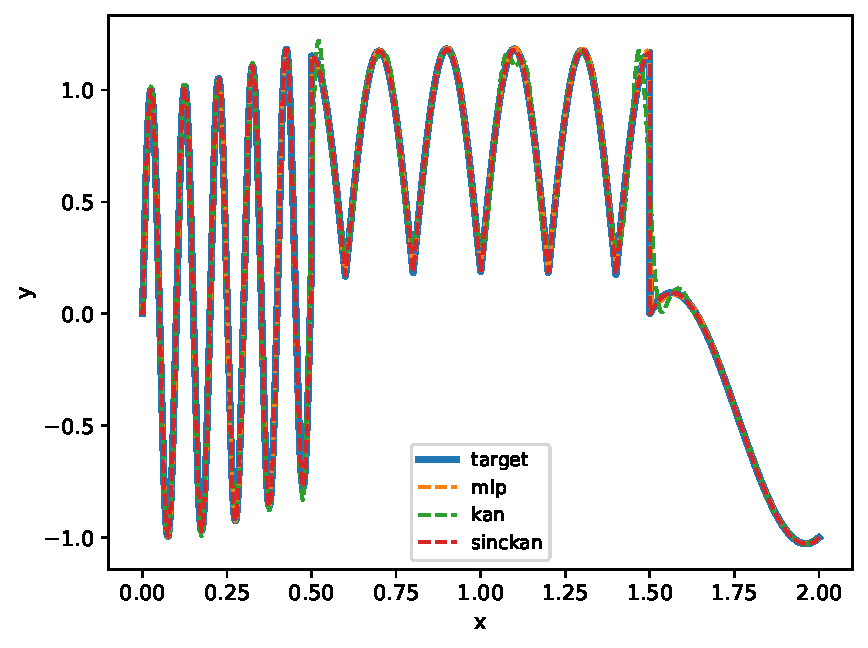
\includegraphics[width=0.3\linewidth]{ThesisFigs/piecewise.pdf}}
    \subfigure[\label{piecewise_error}]{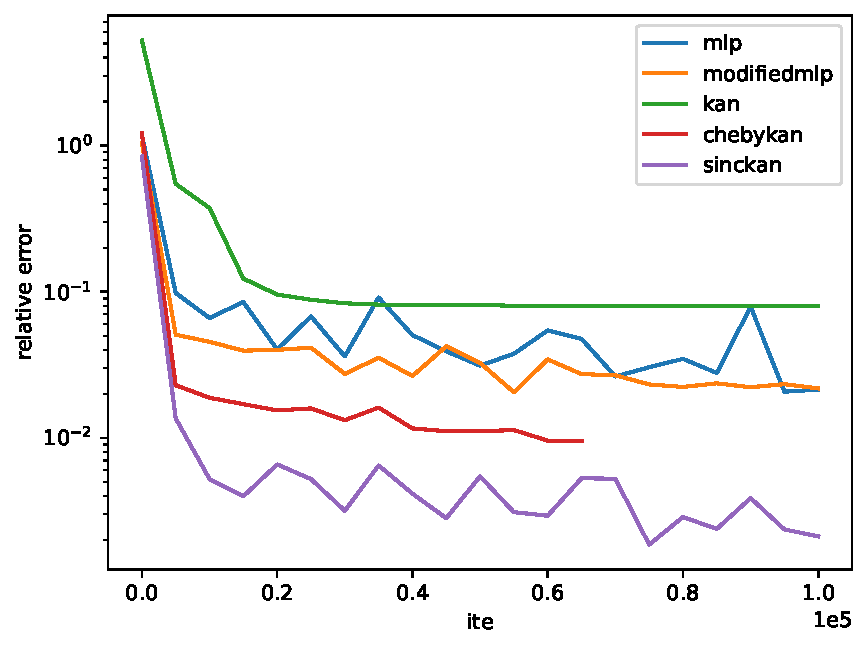
\includegraphics[width=0.3\linewidth]{ThesisFigs/piecewise_error.pdf}}\\
    \subfigure[\label{piecewise_sub1}]{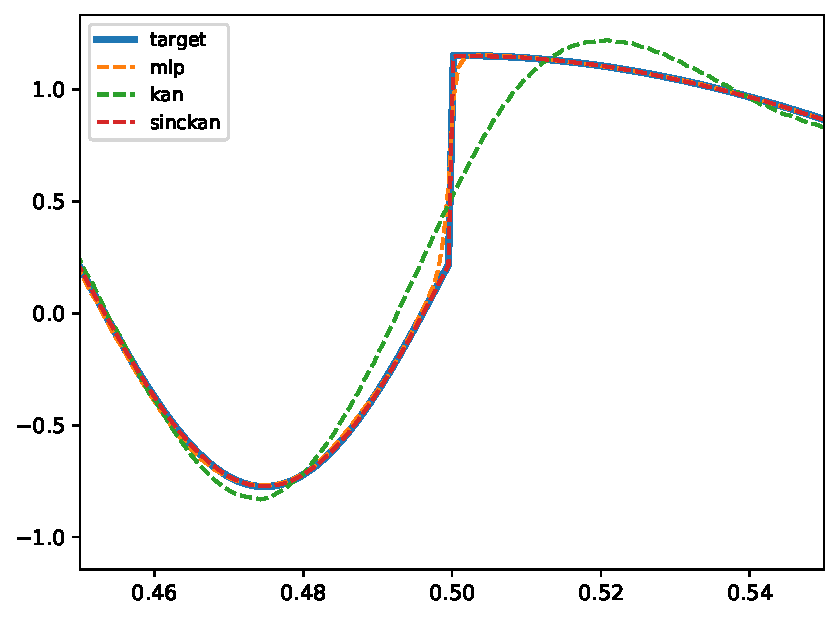
\includegraphics[width=0.3\linewidth]{ThesisFigs/piecewise_sub1.pdf}}
    \subfigure[\label{piecewise_sub2}]{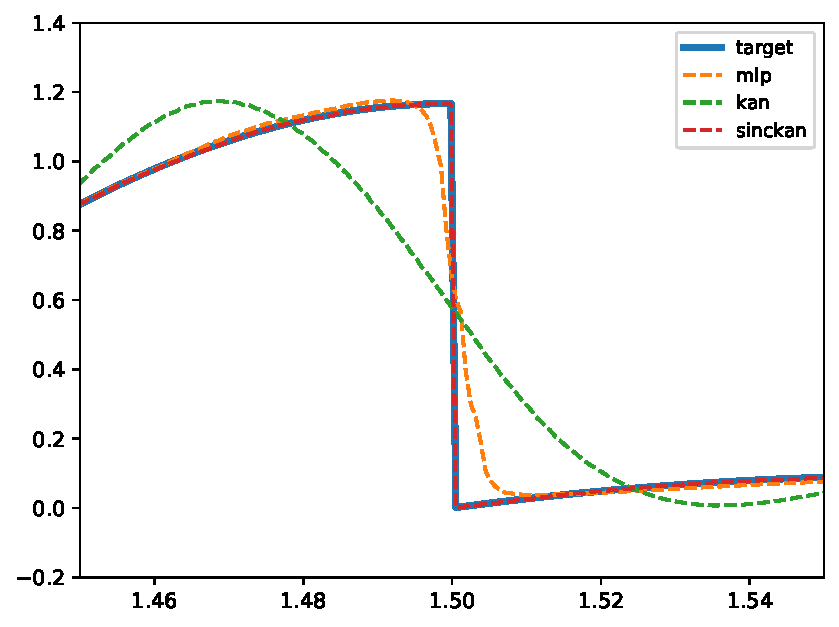
\includegraphics[width=0.3\linewidth]{ThesisFigs/piecewise_sub3.pdf}}
    \caption{\cref{piecewise_solution} depicts the function of \textit{piece-wise} in \cref{table: function approxmation} and compares the performance of SincKAN with MLP and KAN. \cref{piecewise_error} demonstrates the convergence of relative error for all networks, note that although the ChebyKAN we used is the modified ChebyKAN, its training is still unstable. Herein, the results of ChebyKAN in this paper are always the last valid error. \cref{piecewise_sub1} and \cref{piecewise_sub2} demonstrate the singularities in detail and show that the SincKAN can approximate the singularities well while MLP and KAN have obvious differences.}
    \label{fig:enter-label}
\end{figure}
\subsubsection{Step Size Selection Analysis}
The implementation of multiple step sizes $\{h_i\}$ represents a novel methodological contribution specific to SincKAN architecture. To evaluate the efficacy of this approach, we conducted a comprehensive experimental analysis. Let $h_{min}=\min \{h_i\}$ and $h_{max}=\max \{h_i\}$ denote the bounds of the step size range. Based on the theoretical framework presented in Section~\ref{Section: sinckan}, optimal performance should be achieved when the theoretical optimal step size $h^*=\sqrt{\pi d^\star/\beta^\star N}$ lies within the interval $(h_{min}, h_{max})$. 

Our experimental design incorporates two distinct step size sequence formulations, each parameterized by base value $h_0$ and cardinality $M$:

\begin{enumerate}
    \item Inverse decay sequence: $\{h_i\}_{i=1}^{M}$ where $h_i=1/ih_0$
    \item Exponential decay sequence: $\{h_i\}_{i=1}^{M}$ where $h_i=1/h_0^i$
\end{enumerate}

The experimental protocol involved training SincKAN on two representative functions: \textit{sin-low} and \textit{sin-high}. For the inverse decay sequence, we examined $M \in \{1,6,12,24\}$, while the exponential decay sequence was evaluated with $M \in \{1,2,3\}$. Both sequences were tested across base values $h_0 \in \{2.0, \pi, 6.0, 10.0\}$. The number of discretization points $N_{points}$ and degree $N_{degree}$ (where $N_{degree}=2N+1$, with $N$ defined in Equation~\ref{eq: Sinc activation function}) significantly influence SincKAN's performance under different step size configurations. For this analysis, we empirically set $N_{degree}=100$ and $N_{points}=5000$.

The results are illustrated in \cref{fig:select_h_inverse} for inverse decay and \cref{fig:select_h_exp} for exponential decay, and the details including the corresponding error bars are shown in \cref{Appendix: select_h}. For the \textit{sin-low} function, optimal performance (RMSE = $1.49 \times 10^{-4} \pm 8.74 \times 10^{-5}$) was achieved with $h_0=10.0$ and $M=1$. In contrast, the \textit{sin-high} function exhibited superior performance (RMSE = $4.60 \times 10^{-3} \pm 3.70 \times 10^{-4}$) under inverse decay with $h_0=10.0$ and $M=24$. While these functions, characterized by distinctly different Fourier spectra ($4\pi$ and $400\pi$ respectively), yielded divergent optimal hyperparameter configurations, notably accurate approximations for both functions were achieved using inverse decay with $M=6$ and $h_0=10.0$. We also discuss the relationship between degree and data size in \cref{Appendix: scaling law} and the update of basis in \cref{Appendix: update}.

\subsection{Physics-Informed Neural Network Implementation}
The solution of partial differential equations represents a cornerstone of scientific computing, with PINNs emerging as a prominent framework for neural network-based PDE solutions. We demonstrate SincKAN's capabilities through a series of challenging PDE problems. Initial validation involved a selection of classical PDEs to establish SincKAN's robustness, with results presented in Table~\ref{table:pikan_pde}. Detailed problem specifications are provided in Appendix~\ref{Appendix: details of pde}.

\begin{table}[ht]
\caption{Relative L2 error for chosen PDE problems}
\label{table:pikan_pde}
\begin{center}
\begin{adjustbox}{width=\columnwidth, center}
\begin{tabular}{llllll}
\multicolumn{1}{c}{\bf Experiments}  & \multicolumn{1}{c}{\bf MLP} & \multicolumn{1}{c}{\bf modified MLP} &\multicolumn{1}{c}{\bf KAN} & \multicolumn{1}{c}{\bf ChebyKAN} & \multicolumn{1}{c}{\bf SincKAN (ours)} 
\\ \hline  
\textit{perturbed} & $2.89e\mbox{-}2\pm 3.09e\mbox{-}2$ & $6.30e\mbox{-}1\pm1.14e\mbox{-}1$ &  $4.48e\mbox{-}3 \pm 4.20e\mbox{-}3 $& $6.73e\mbox{-}1 \pm 1.02e\mbox{-}1 $& \color{red}{$1.88e\mbox{-}3 \pm 8.55e\mbox{-}4$} \\ 
\textit{nonlinear} & $3.92e\mbox{-}1 \pm 2.36e\mbox{-}5$ & $1.56e\mbox{-}2 \pm 2.10e\mbox{-}2$ & \color{red}{$6.15e\mbox{-}4 \pm 7.96e\mbox{-}4$} & $7.78e\mbox{-}1 \pm 2.67e\mbox{-}2$  & $1.77e\mbox{-}3 \pm 1.06e\mbox{-}3$ \\ 
\textit{bl-2d} & $2.38e\mbox{-}1\pm6.22e\mbox{-}2$ & $5.34e\mbox{-}2 \pm 1.91e\mbox{-}2$ &$1.19e\mbox{-}2 \pm 4.22e\mbox{-}3$ & $5.97e\mbox{-}2\pm 3.83e\mbox{-}2$ & \color{red}{$2.31e\mbox{-}3\pm7.10e\mbox{-}4$} \\
\textit{ns-tg-u} & $8.14e\mbox{-}5 \pm 1.96e\mbox{-}6$ & \color{red}{$2.14e\mbox{-}5 \pm 2.67e\mbox{-}6$} & $3.21e\mbox{-}4 \pm 2.02e\mbox{-}5$ & $6.43e\mbox{-}2 \pm 2.70e\mbox{-}2$& $6.51e\mbox{-}4 \pm 7.03e\mbox{-}5$\\      
\textit{ns-tg-v} & $8.30e\mbox{-}5 \pm 2.47e\mbox{-}6$ & \color{red}{$1.91e\mbox{-}5 \pm 1.63e\mbox{-}6$} & $4.04e\mbox{-}4 \pm 1.25e\mbox{-}4$ & $5.86e\mbox{-}2 \pm 4.15e\mbox{-}2$& $1.34e\mbox{-}3 \pm 4.38e\mbox{-}4$
\end{tabular}
\end{adjustbox}
\end{center}
\end{table}

\begin{figure}[ht]
  \centering
  \subfigure[\label{bl_solution_sinckan}Solution comparison]{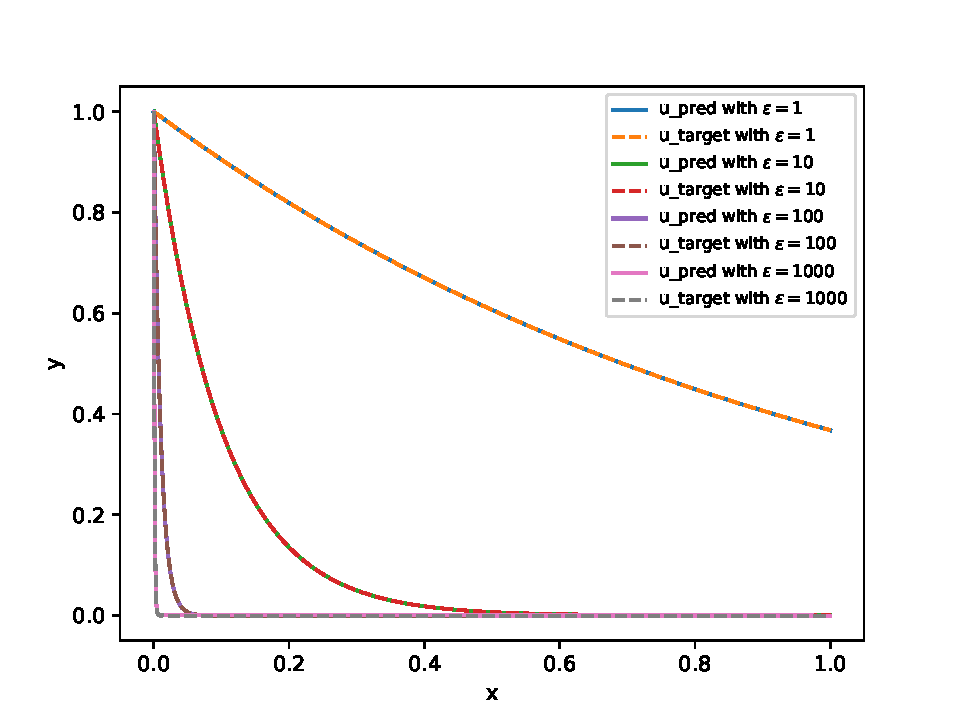
\includegraphics[width=0.3\linewidth]{ThesisFigs/bl_solution_sinckan.pdf}}
  \subfigure[\label{bl_loss_sinckan}Loss convergence]{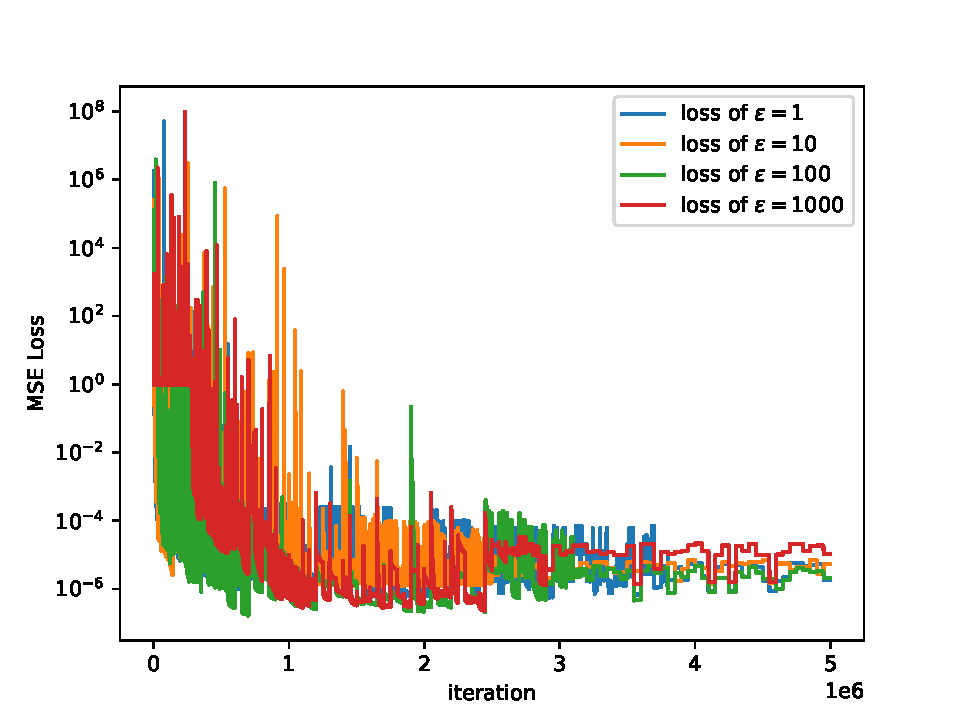
\includegraphics[width=0.3\linewidth]{ThesisFigs/bl_loss_sinckan.pdf}}
  \subfigure[\label{bl_1000_sinckan}High-$\epsilon$ performance]{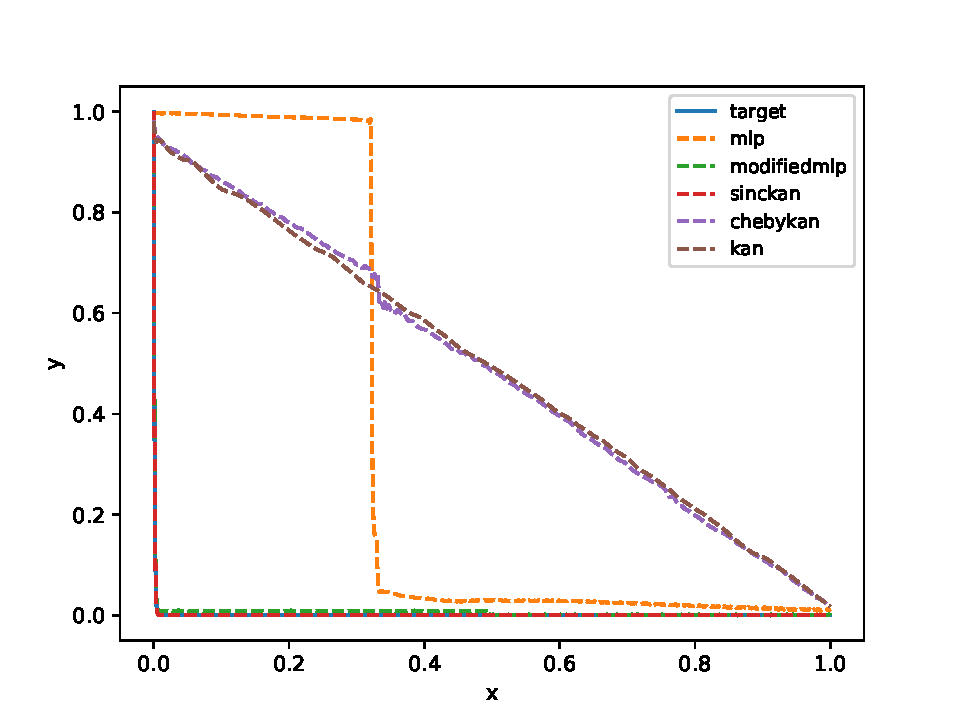
\includegraphics[width=0.3\linewidth]{ThesisFigs/bl_1000_sinckan.pdf}}
  \caption{Analysis of boundary layer problem: (a) Comparison between exact solutions and SincKAN predictions for various $\epsilon$ values, demonstrating robust performance even with extremely narrow boundary layers; (b) Training loss convergence patterns across different $\epsilon$ values; (c) Comparative performance analysis for $\epsilon=1000$, illustrating superior SincKAN performance in cases where traditional architectures struggle with large derivatives in the boundary layer.}
  \label{fig:bl_sinckan}
\end{figure}

\subsubsection{Analysis of Boundary Layer Problems}
To provide a comprehensive demonstration of SincKAN's capabilities relative to existing architectures, we conducted an in-depth analysis of the boundary layer problem:
\begin{equation} \label
{eq: bl}
u_{xx}/\epsilon+u_{x}=0, \quad x \in
 [0,1]
\end{equation}
with exact solution $u(x)=\exp (-\epsilon x)$. The parameter $\epsilon$ controls the width of the boundary layer, with increasing values of $\epsilon$ corresponding to decreasing boundary layer width and consequently increasing learning complexity. Table~\ref{table:bl_pikan} presents a comparative analysis across different values of $\epsilon$, while Figure~\ref{fig:bl_sinckan}
 provides detailed visualization of the results.

\begin{table}[ht]
\caption{Relative L2 error for different $\epsilon$ in \cref{eq: bl}}
\label{table:bl_pikan}
\begin{center}
\begin{adjustbox}{width=\columnwidth, center}
\begin{tabular}{llllll}
\multicolumn{1}{c}{\bf $\epsilon$ } & \multicolumn{1}{c}{\bf MLP} & \multicolumn{1}{c}{\bf Modified MLP} &\multicolumn{1}{c}{\bf KAN} &\multicolumn{1}{c}{\bf ChebyKAN} & \multicolumn{1}{c}{\bf SincKAN (ours)} 
\\ \hline 
1    & $ 6.60e\mbox{-}5 \pm 1.91e\mbox{-}5 $ &$ 3.88e\mbox{-}6 \pm 7.22e\mbox{-}7 $   & $ 5.97e\mbox{-}6 \pm 5.24e\mbox{-}6 $ & \color{red}{$ 1.98e\mbox{-}6 \pm 4.51e\mbox{-}7 $} & $ 7.78e\mbox{-}5 \pm 1.14e\mbox{-}4 $ \\
10   & $ 2.83e\mbox{-}4 \pm 4.22e\mbox{-}5 $& $ 1.69e\mbox{-}4 \pm 6.85e\mbox{-}5 $ &$ 3.23e\mbox{-}5 \pm 1.81e\mbox{-}5 $ & \color{red}{$4.45e\mbox{-}6 \pm 4.01e\mbox{-}7$} & $1.14e\mbox{-}4 \pm 1.64e\mbox{-}4 $\\
$10^2$  & $ 1.29e\mbox{-}3 \pm 3.24e\mbox{-}4 $& $ 6.25e\mbox{-}4 \pm 2.27e\mbox{-}4 $ & $ 1.25e\mbox{-}2 \pm 2.62e\mbox{-}3 $ & $ 5.27e\mbox{-}4 \pm 6.55e\mbox{-}4 $& \color{red}{$1.68e\mbox{-}4 \pm 6.16e\mbox{-}5$} \\
$10^3$ &$ 9.87 \pm 8.70 $ & $ 1.53e\mbox{-}1 \pm 5.59e\mbox{-}2 $    & $ 11.3 \pm 8.79 $ & $ 10.9 \pm 7.18 $ & \color{red}{$5.48e\mbox{-}3 \pm 3.45e\mbox{-}3$}\\
\textcolor{blue}{$10^4$} &$ 8.41 \pm 3.64 $ & $ 6.52 \pm 4.35 $    & $ 9.73 \pm 8.77 $ & $ 22.1 \pm 4.49 $ & \color{red}{$5.27e\mbox{-}3 \pm 1.29e\mbox{-}3$}
\end{tabular}
\end{adjustbox}
\end{center}
\end{table}

\subsubsection{Analysis of Fractional PDEs}
Fractional partial differential equations present significant computational challenges, with traditional numerical methods still struggling to address their non-local nature and inherent singularities. We examine the fractional PDE:
\begin{equation}
    -\Delta^su+\gamma u=f, \quad x\in
 (-1,1),
\end{equation}
where $f=1+\gamma u$
, with solution:
\begin{equation}
    u(x)=\frac{2^{-2s}\Gamma(d/2)}{\Gamma(d/2+s)\Gamma(1+s)}(1-\|x\|
^2_2)^s.
\end{equation}

Figure~\ref{fig:frac}
 presents our comparative analysis results. The superior performance of SincKAN in handling the inherent singularities of fractional PDEs is particularly evident in the convergence patterns and error distributions.

\begin{figure}[ht]
  \centering
  \subfigure[\label{frac_loss}Loss convergence]{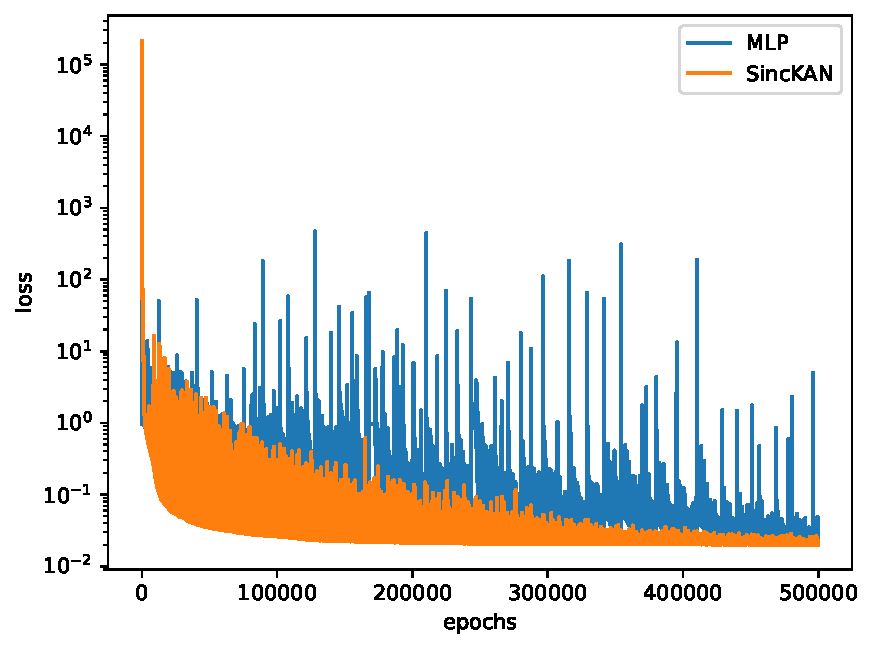
\includegraphics[width=0.3\linewidth]{ThesisFigs/frac_loss85_1.pdf}}
  \subfigure[\label{frac_error85}Error analysis ($s=0.85$)]{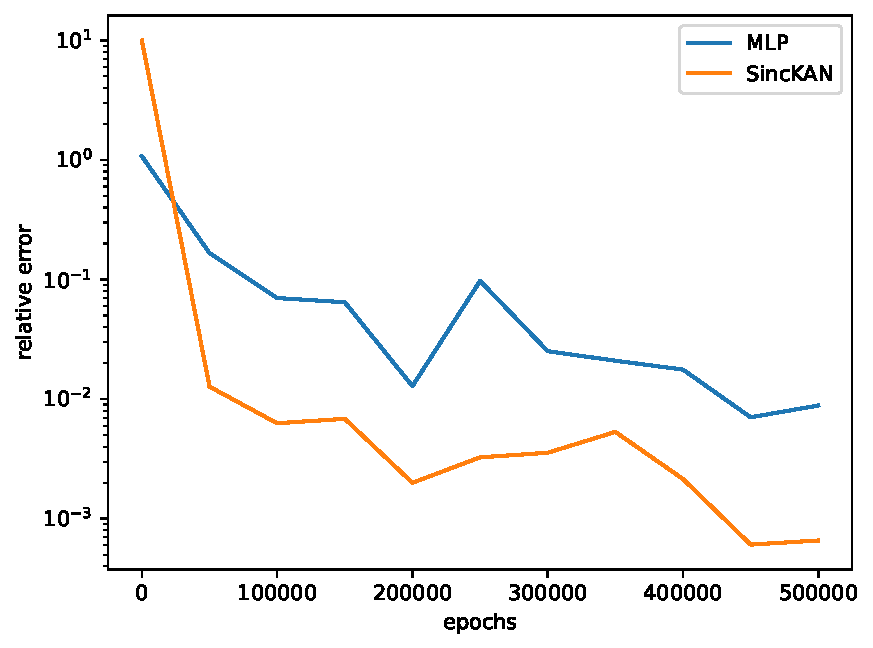
\includegraphics[width=0.3\linewidth]{ThesisFigs/frac_error85_1.pdf}}
  \subfigure[\label{frac_error95}Error analysis ($s=0.95$)]{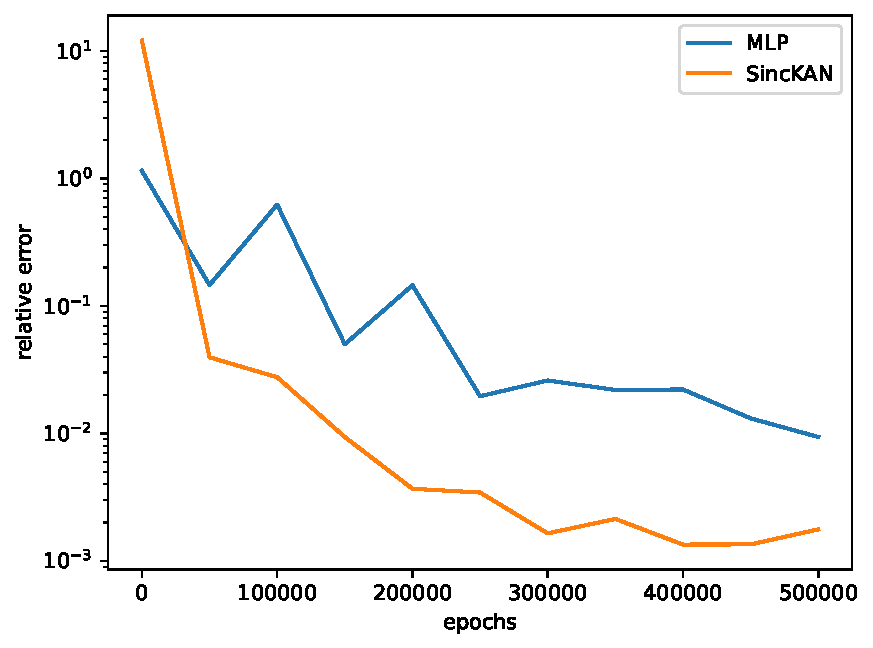
\includegraphics[width=0.3\linewidth]{ThesisFigs/frac_error95_1.pdf}}
  \caption{Fractional PDE analysis: (a) Comparative loss convergence between MLP and SincKAN for $s=0.85$; (b,c) Error distribution analysis for $s=0.85$ and $s=0.95$ respectively, demonstrating SincKAN's superior handling of fractional-order derivatives.}
  \label{fig:frac}
\end{figure}

\subsubsection{High-Dimensional Problem Analysis}
To evaluate scalability, we examined the classical high-dimensional Poisson equation:
\begin{equation}
    \Delta u =f, \quad \boldsymbol{x}\in
 [0,1]^d,
\end{equation}
with source term $f=2\alpha(2\alpha \|\boldsymbol{x}\|^2_2-d) e^{-\alpha \|\boldsymbol{x}\|_2^2}$, yielding the exact solution $u(\boldsymbol{x})=e^{-\alpha \|\boldsymbol{x}\|^2_2}$. Our experiments focused on the challenging case of $d=100$ dimensions, with detailed experimental parameters provided in Appendix~\ref{Appendix: expeirment details}
.

\begin{figure}[ht]
  \centering
  \subfigure[\label{high_distribution}Point distribution]{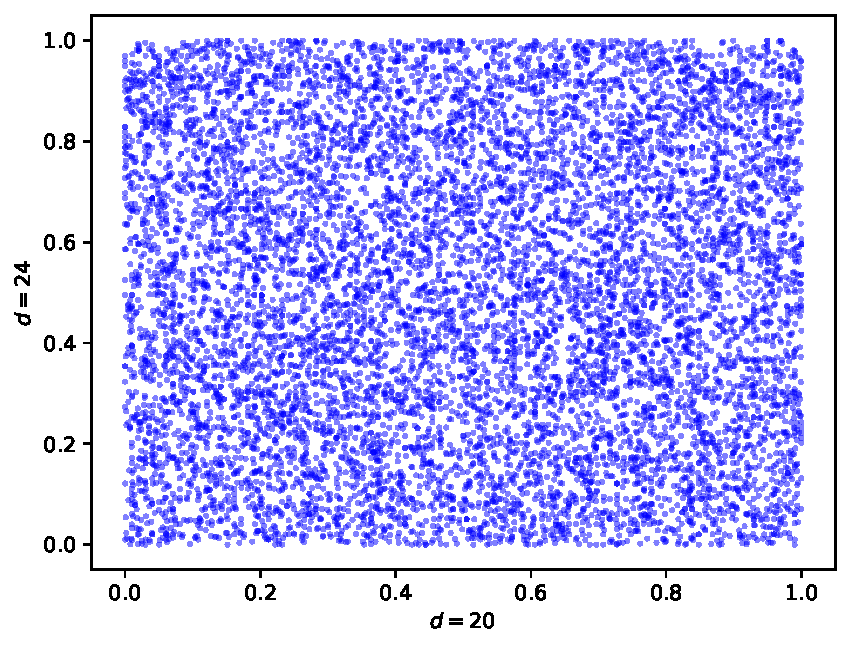
\includegraphics[width=0.3\linewidth]{ThesisFigs/points_distribution.pdf}}
  \subfigure[\label{high_mlp}MLP error analysis]{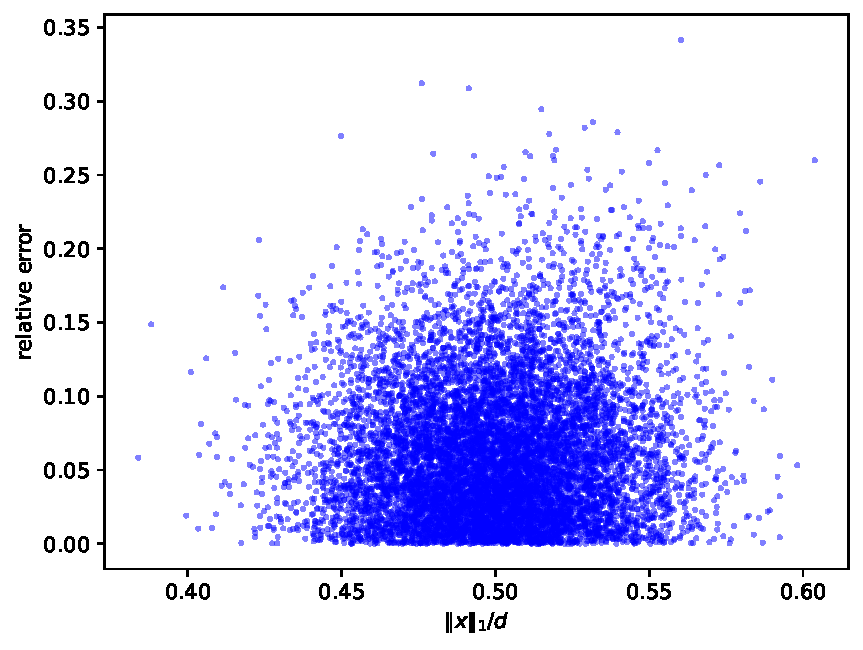
\includegraphics[width=0.3\linewidth]{ThesisFigs/high-dim_mlp.pdf}}
  \subfigure[\label{high_sinckan}SincKAN error analysis]{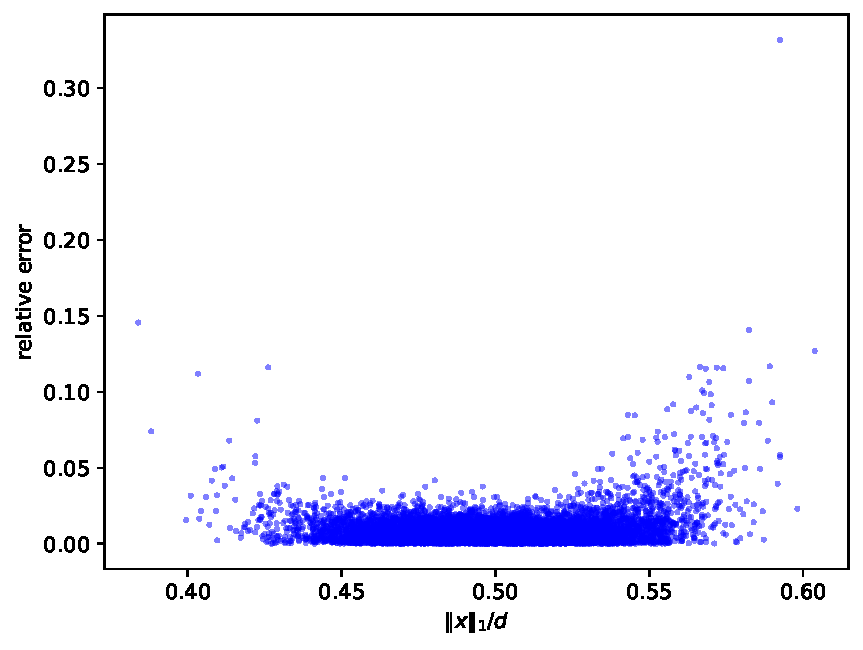
\includegraphics[width=0.3\linewidth]{ThesisFigs/high-dim_sinckan.pdf}}
  \caption{High-dimensional analysis: (a) Distribution visualization of test points in dimensions 20 and 24; (b,c) Comparative error analysis between MLP and SincKAN implementations, demonstrating SincKAN's superior performance in high-dimensional spaces.}
  \label{fig:high_dim}
\end{figure}

\subsubsection{Ablation Studies}
To systematically evaluate the architectural contributions of SincKAN, we conducted comprehensive ablation studies examining two key components: the normalized transformation and the linear skip connection. While Sinc numerical methods traditionally employ various coordinate transformations, and KANs incorporate skip connections with SiLU functions, our implementation introduces specific modifications to these elements. To rigorously assess the impact of these modifications, we performed comparative analyses using two representative test cases: Burger's equation (Equation~\ref{eq:burgers}) and the time-dependent nonlinear equation (Equation~\ref{eq:tnonlinear}
).

\begin{table}[ht]
\caption{Relative L2 error for ablation study}
\label{table:ablation}
\begin{center}
\begin{adjustbox}{width=0.5\columnwidth, center}
\begin{tabular}{ccccll}
\multicolumn{1}{c} {$\psi$}  & \multicolumn{1}{c}{$\gamma$} & \multicolumn{1}{c}{\bf Linear }  &\multicolumn{1}{c}{\bf SiLU} & \multicolumn{1}{c}{\bf T-nonlinear} & \multicolumn{1}{c}{\bf Burgers' equation}
\\ \hline  
\ding{56} & \ding{56} & \ding{56} & \ding{56} & $9.20e\mbox{-}4\pm4.31e\mbox{-}4$ & $1.57e\mbox{-}2\pm4.31e\mbox{-}3$\\
\ding{56} & \ding{52} & \ding{56} & \ding{56} &  $5.80e\mbox{-}4\pm1.89e\mbox{-}4$ &\color{red}{$6.21e\mbox{-}4\pm1.96e\mbox{-}4$}\\
\ding{56} & \ding{52} & \ding{52} & \ding{56} & $2.44e\mbox{-}4\pm6.08e\mbox{-}5$ & $3.12e\mbox{-}3\pm2.48e\mbox{-}3$ \\
\ding{56} & \ding{52} & \ding{56} & \ding{52} & \color{red}{$1.60e\mbox{-}4\pm3.17e\mbox{-}5$} & $8.90e\mbox{-}3\pm6.76e\mbox{-}3$ \\
\ding{52} & \ding{56} & \ding{52} & \ding{56} & $1.11e\mbox{-}2\pm1.17e\mbox{-}3$& $7.36e\mbox{-}2\pm2.02e\mbox{-}2$ \\
\ding{52} & \ding{56} & \ding{56} & \ding{52} & $1.30e\mbox{-}2\pm4.00e\mbox{-}4$ & $1.12e\mbox{-}1\pm6.80e\mbox{-}3$ \\
\end{tabular}
\end{adjustbox}
\end{center}
\end{table}

Table~\ref{table:ablation} presents our ablation study results, where $\psi(x)=\log(\frac{x-a}{b-x})$ represents the traditional transformation, $\gamma(x)=\tanh(x)$ denotes our normalized transformation, $\mathrm{Linear}(x)=w_1x+w_2+\phi(x)$ represents the linear skip connection, and $\mathrm{SiLU}(x)=w_b\mathrm{silu}(x)+w_s\phi(x)$
 indicates the SiLU skip connection. The results reveal several significant findings:

First, the non-normalized transformation consistently demonstrates inferior performance compared to configurations without transformations, highlighting the importance of proper normalization in neural network architectures. Second, while the linear skip connection may not achieve optimal performance for both equations individually, it exhibits superior stability characteristics in the SincKAN framework, suggesting its value as a robust architectural component.

\section{Conclusion}\label{Section: conclusion}
This research introduces Sinc Kolmogorov-Arnold Networks (SincKANs), a novel neural network architecture that leverages the powerful approximation capabilities of Sinc functions within the KAN framework. By implementing Sinc functions for activation function interpolation, SincKANs inherit and enhance the ability to handle singularities effectively. To address the challenges of optimal step size selection, we introduced multi-$h$
 interpolation, which our experimental results indicate is fundamental to SincKAN's superior performance in approximating complex smooth functions.

The implementation challenges were systematically addressed through three key innovations: (1) the introduction of normalized transformation to prevent convergence issues, (2) the implementation of skip-connections with learnable linear functions to satisfy decay conditions, and (3) the development of multi-step size interpolation methodology. These modifications collectively enable SincKANs to serve as a competitive alternative to existing neural network architectures in the PINN framework.

Our experimental validation began with function approximation tasks, where SincKANs demonstrated superior performance across diverse test cases. However, we acknowledge that direct function approximation rarely represents the primary objective in machine learning applications. Following this validation, we evaluated SincKAN performance in PDE solution tasks within the PINN framework. While SincKANs achieved impressive approximation accuracy across all tested PDEs, their optimal performance was particularly evident in boundary layer problems, though some oscillation effects were observed due to derivative approximation challenges.

\textbf{Limitations}: The accuracy of derivative approximation using Sinc numerical methods exhibits inherent limitations near Sinc end-points. While various solutions have been proposed in the literature, such as Lagrange polynomial approximation \citep{stenger2009polynomial} and discrete function substitution \citep{wu2006sinc}, these approaches have not yet been successfully adapted to the SincKAN architecture for PINN applications. To mitigate accuracy issues, we employed conservative parameter settings ($h_0$, $M$, and $N$), which, while enabling successful PDE solution, potentially limit SincKAN's full capabilities (detailed oscillation analysis provided in Appendix~\ref{Appendix: oscillation}
). These limitations particularly affect high-order problems such as Korteweg–De Vries and Kuramoto–Sivashinsky equations.

\textbf{Future Directions}: Several promising research directions emerge from our findings. For PDEs requiring only first derivatives, SincKAN can potentially utilize larger parameter values ($h_0$, $M$, and $N$), potentially improving performance. The mixed residual method approach of MIM \citep{lyu2022mim,li2024priori}, which transforms high-order PDEs into first-order PDE systems, presents a promising avenue for extending SincKAN capabilities to higher-order problems. Additionally, alternative differentiation approaches \citep{cen2024deep,yu2024fourier}
 warrant investigation as potential replacements for automatic differentiation in the SincKAN framework.

% ------------------------------------------------------------------------

%%% Local Variables: 
%%% mode: latex
%%% TeX-master: "../thesis"
%%% End: 
